\chapter{Systems of Differential Equations}

\section{Matrices and Linear Systems}
\begin{problem}
   Consider the second order differential equation 
    \[ x'' + bx' + c x = 0 \]
    By substituting $y = x'$ we can get a system of differential equations.  What is the
    system, write it as a matrix equation, and what is the meaning of $y$ in this system? 
\end{problem}
\solution{
    \begin{flalign*}
        x' &= y \\
        y' &= -by-cx
    \end{flalign*}
    \[ \frac{d\bx}{dt} = \begin{pmatrix} 0 & 1 \\ -c & -b \end{pmatrix} \bx \]
}



\begin{problem}   
    If 
    \[ \left\{ \begin{array}{cl} x' &= y \\ y' &= -5x-2y \end{array} \right. \]
    Then what was the mass spring system associated with the system?  Draw a picture of
    the solutions to $x$ and $y$.
\end{problem}
\solution{
    \begin{flalign*}
        x'' + 2x'+5x=0
    \end{flalign*}
    Observe that $b^2-4mk = 4-4(5) < 0$ so the system is underdamped and will
    oscilalte.  Show in PPlane.
}

\begin{problem}
    In the previous problem you likely arrived at the second order differential equation
    $x'' + 2x' + 5x = 0$.  The discriminant on this differential equation is
    $b^2-4mk=4-4(1)(5)=-16$ so we know that the system is underdamped.  
    \begin{enumerate}
        \item[(a)] What are the roots of the characteristic polynomial.
        \item[(b)] Using the system in the previous problem write the associated matrix
            equation and find the eigenvalues of the matrix.  What do you notice?
        \item[(c)] Make a conjecture about the roots of the characteristic polynomial and
            the eigenvalues of the associated matrix.
    \end{enumerate}
\end{problem}

\begin{problem}
    Consider the second order differential equation modeling a spring-mass system: 
    \[ x'' + 2x' + 2x = 0. \]
    \begin{enumerate}
        \item[(a)] Find the discriminant, the roots of the characteristic polynomial,
            classify the system, and discuss the expected behavior.
            \solution{The system is underdamped since $b^2-4mk<0$.  Hence, the system will
            exhibit long-term damped oscillations.  The roots of the characteristic
        polynomial are 
        \[ r = \frac{-2 \pm \sqrt{4-4(1)(2)}}{2} = -1 \pm i \]
        }
        \item[(b)] Write the differential equation as a first order system and find the
            associated matrix equation.
            \solution{
            \[ \begin{pmatrix} x' \\ y' \end{pmatrix} = \begin{pmatrix} 0 & 1 \\ -2 & -2
                \end{pmatrix} \begin{pmatrix} x \\ y \end{pmatrix}. \]
            }
        \item[(c)] Find the eigenstructure of $A$ and discuss what this means about the
            behavior of the system.
    \end{enumerate}
\end{problem}

\begin{thm}
    If we transform the second order differential equation $x'' + bx' + cx =0$ into the
    first order matrix equation $\begin{pmatrix} x' \\ y' \end{pmatrix} = \begin{pmatrix}
        0 & 1 \\ -c & -b \end{pmatrix} \begin{pmatrix} x \\ y \end{pmatrix}$ by making the
            substitution $y = x'$ then the roots of the characteristic polynomial $p(r) = r^2 +
            br + c$ are the same as the eigenvalues of the matrix in the first-order
            system.
\end{thm}
\begin{proof}
    Let $A = \begin{pmatrix} 0 & 1 \\ -c & -b \end{pmatrix}$ and observe that $\det(A
        -\lambda I) = \lambda^2 + \lambda b + c$.  The result follows.  \\ (The reader
        should fill in all of the details of this proof.) 
\end{proof}


\begin{problem}
    Consider a two-tank system where brine is transferred between them according to the
    following rules.
    \begin{itemize}
        \item 20 L/min of fresh water enters Tank \#1
        \item Tank \#1 holds $x(t)$ kg of salt and holds a total of 100 liters of total
            mixture.
        \item Tank \#2 holds $y(t)$ kg of salt and holds a total of 200 liters of total
            mixture.
        \item Mixture runs from Tank \#1 to Tank \#2 at a rate of 30 L/min.
        \item Mixture runs from Tank \#2 to Tank \#1 at a rate of 10 L/min.
        \item Tank \#2 drains mixture at a rate of 20 L/min
    \end{itemize}
    Write a system of differential equations modeling the transfer of brine in this
    two-tank system.  What interesting questions can you ask about this system?  Finally,
    write the system as a matrix equation. You may want to investigate the system using
    software like \texttt{pplane}.
\end{problem}
\solution{
    \begin{flalign*}
        \frac{dx_1}{dt} &= \text{rate in from $x_2$} - \text{rate out to $x_2$} +
        \text{rate in from external} \\
        \frac{dx_2}{dt} &= \text{rate in from $x_1$} - \text{rate out to $x_1$} +
        \text{rate out to external} 
    \end{flalign*}
    Using concentrations in each we get
    \begin{flalign*}
        \frac{dx_1}{dt} &= -\frac{30}{100} x_1 + \frac{10}{200} x_2 + 0  =
        -\frac{3}{10} x_1 - \frac{1}{20}x_2 \\
        \frac{dx_2}{dt} &= \frac{30}{100} x_1 - \frac{10}{200} x_2 - \frac{20}{200} x_2 =
        \frac{3}{10} x_1 - \frac{3}{20} x_2
    \end{flalign*}
    Show using PPlane as well as get sketches of the time solutions.
}



\begin{problem}
    Three 100 gallon fermentation tanks are connected as shown below, and the mixtures in
    each tank are kept uniform by stirring.  Denote $x_j(t)$ as the amount of alcohol in
    tank $T_j$ at time $t$.  Suppose that the mixture circulates between the tanks at the
    rate of 10 gal/min.  What system of differential equations governs this closed system?
    Write the system as a matrix equation.
\end{problem}
\solution{
    \[ \frac{d\bx}{dt} = \frac{1}{10} \begin{pmatrix} -1 & 0 & 1 \\ 1 & -1 & 0 \\ 0 &
        1 & -1 \end{pmatrix} \bx \]
}
\begin{center}
    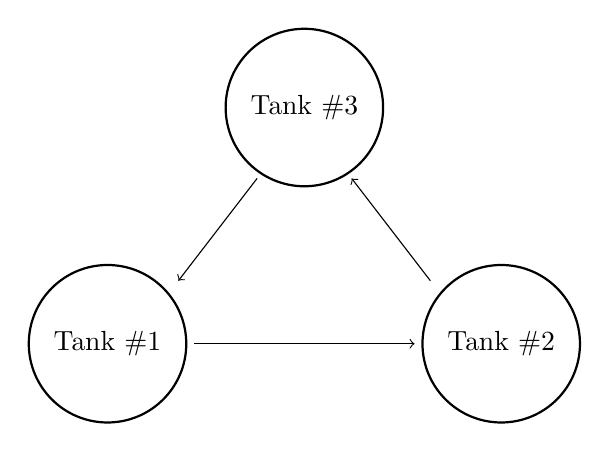
\begin{tikzpicture}
        \draw[black, thick] (0,0) node{Tank \#1} circle(1cm);
        \draw[black, thick] (5,0) node{Tank \#2} circle(1cm);
        \draw[black, thick] (2.5,3) node{Tank \#3} circle(1cm);
        \draw[->] (1.1,0) -- (3.9,0);
        \draw[->] (4.1,0.8) -- (3.1,2.1);
        \draw[->] (1.9,2.1) -- (0.9,0.8);
    \end{tikzpicture}
\end{center}



\begin{problem}
\item A coupled spring mass system is shown below.  Let $x_1(t)$ denote the displacement of
    mass 1 from its equilibrium and let $x_2(t)$ denote the displacement of mass 2 from
    its equilibrium.  Assuming no damping forces
    complete the system of differential equations below.


        \begin{center}
            \begin{tikzpicture}
                \tikzstyle{ground}=[fill,pattern=north east lines,draw=none,minimum width=0.3,minimum height=0.6]
                \tikzstyle{sky}=[fill,pattern=north east lines,draw=none,minimum width=0.3,minimum height=0.6]

                \node (wall1) [ground, minimum height=2cm] {};
                \draw (wall1.north east) -- (wall1.south east);
                \node [draw,minimum width=0.5cm,minimum height=0.5cm] (massF) at (3,0)
                {$M_1$};
                \node [draw,minimum width=0.5cm,minimum height=0.5cm] (massG) at (7,0)
                {$M_2$};
                \draw [
                    snake=coil,
                    segment amplitude=5pt,
                    segment length=5pt
                ] (wall1.east) -- (massF); 
                \draw [
                    snake=coil,
                    segment amplitude=5pt,
                    segment length=5pt
                ] (massF.east) -- (massG.west); 
                \draw [
                    thick,
                    decoration={
                        brace,
                        mirror,
                        raise=0.5cm
                    },
                    decorate
                ] (wall1.east) -- (massF) 
                node [pos=0.5,anchor=north,yshift=-0.55cm] {$k1$}; 
                \draw [
                    thick,
                    decoration={
                        brace,
                        mirror,
                        raise=0.5cm
                    },
                    decorate
                ] (massF.east) -- (massG.west) 
                node [pos=0.5,anchor=north,yshift=-0.55cm] {$k2$}; 
            \end{tikzpicture}
        \end{center}
% 
%     \begin{center}
%         \includegraphics[width=0.6\columnwidth]{CoupledSpringMass}
%     \end{center}
    \begin{flalign*}
        m_1 x_1 '' &= -\underline{\hspace{0.5in}} x_1 + k_2 \underline{\hspace{0.5in}} \\
        m_2 x_2 '' &= -\underline{\hspace{0.5in}} \left( x_2 - x_1 \right)
    \end{flalign*}
    Once you have the system, write it as a matrix equation.
\end{problem}
\solution{
    \begin{flalign*}
        m_1 x_1 '' &= -k_1 x_1 + k_2 (x_2 - x_1) = -(k_1+k_2)x_1 + k_2 x_2 \\
        m_2 x_2 '' &= -k_2 \left( x_2 - x_1 \right) = k_2 x_1 - k_2 x_2
    \end{flalign*}
    \[ \frac{d^2 \bx}{dt^2} = \begin{pmatrix} -(k_1+k_2) & k_2 \\ k_2 & -k_2 \end{pmatrix}
    \bx \]
}

\begin{problem}
    The previous problem ended in a $2\times 2$ second order system.  Make an appropriate
    substitution and arrive at a $4\times 4$ first order system.  
\end{problem}
\solution{
Let $y_1 = x_1'$ and $y_2 = x_2'$.  Therefore,
\begin{flalign*}
    m_1 y_1' &= -(k_1+k_2)x_1 + k_2 x_2 \\
    x_1' &= y_1 \\
    m_2 y_2' &= k_2 x_1 - k_2 x_2\\
    x_2' &= y_2
\end{flalign*}
\[ \begin{pmatrix} y_1' \\ x_1' \\ y_2' \\ x_2' \end{pmatrix} = \begin{pmatrix} 0 &  -(k_1 +
        k_2) & 0 & k_2 \\
        1 & 0 & 0 & 0 \\
        0 & k_2 & 0 & -k_2 \\
        0 & 0 & 1 & 0 \end{pmatrix} \begin{pmatrix} y_1 \\ x_1 \\ y_2 \\ x_2 \end{pmatrix}
\]
}


% \begin{problem}
%     \begin{itemize}
%             \input{ClickerQuestions/DEQ.10.18.070}
%     \end{itemize}
% \end{problem}



\section{The Eigenvalue Method for Linear Systems}
Now let's interweave the idea of eigenvalues in with systems of differential equations. As
we already know, the eigenvalues and eigenvectors of a matrix $A$ tell us the underlying
structure of the matrix.  In some sense they are the DNA of the matrix.  In the cases that
we investigate here the eigen-structure of $A$ will tell us about the solution curves of
the linear first order differential equation.

\begin{thm}\label{thm:eigen_ode}
    Let $\lambda$ be an eigenvalue of the matrix $A$ for the first
    order linear system 
    \[ \frac{d\bx}{dt} = A \bx. \]
    If $\bv$ is an eigenvector associated with eigenvalue $\lambda$ then 
    \[ \bx(t) = \bv e^{\lambda t} \]
    is a nontrivial solution of the system.
\end{thm}
\begin{proof}
    Let $A$ be a real square matrix and let $\bv$ and $\lambda$ be an eigen-pair for $A$.
    To check that $\bx = \bv e^{\lambda t}$ is a solution to the differential equation
    $\bx' = A\bx$ we substitute $\bx$ in on both sides and check.

    On the left-hand side of the differential equation we get
    \begin{flalign*}
        \frac{d\bx}{dt} = \frac{d}{dt} \left( \bv e^{\lambda t} \right) 
        = \bv \frac{d}{dt} \left( e^{\lambda t} \right) 
        = \bv \left( \lambda e^{\lambda t} \right) 
        = \lambda e^{\lambda t} \bv.
    \end{flalign*}
    On the right-hand side of the differential equation we get
    \begin{flalign*}
        A\bx = A \left( \bv e^{\lambda t} \right) 
        = e^{\lambda t} A \bv 
        = e^{\lambda t} \left( \lambda \bv \right) 
        = \lambda e^{\lambda t} \bv \quad \checkmark.
    \end{flalign*}
\end{proof}

\begin{thm}
    If $\bv_1, \bv_2, \dots, \bv_k$ are unique solutions to the first
    order linear system of equations
    $\bx'=A\bx$ then a linear combination 
    \[ \bv = \sum_{j=1}^k c_j \bv_j \]
    is also a solution of $\bx' = A \bx$.
\end{thm}
\begin{proof}
    Since the differential equation is linear we know that a linear combination of
    solutions is also a solution.  
\end{proof}

\begin{thm}
    If the matrix $A$ has eigenvectors $\bv_1, \bv_2, \ldots, \bv_n$ and associated
    eigenvectors $\lambda_1, \lambda_2, \ldots, \lambda_n$ then the general solution to
    the differential equation $\bx' = A \bx$ is
    \[ \bx(t) = \underline{\hspace{2in}} \]
\end{thm}
\begin{proof}
    (Fill in the blank above and prove the theorem)
\end{proof}
\solution{
    \[ \bx(t) =c_1 \bv_1 e^{\lambda_1 t} +c_2 \bv_2 e^{\lambda_2 t} + \cdots +c_k \bv_k
    e^{\lambda_k t} \]
    This follows immediately from the previous two theorems.
}

% \begin{problem}
%     Considering the previous two theorems, if
%     \[ \frac{d\bx}{dt} = A \bx \]
%     then what is the solution to the system?
% \end{problem}

\begin{problem}
    Solve the following linear system of differential equations.
    \begin{flalign*}
        x_1' &= 4x_1 - x_2 \\
        x_2' &= 2x_1 + x_2
    \end{flalign*}
    with initial conditions $x_1(0) = 1$ and $x_2(0) = 3$. Complete the problem by giving a plots
    $x_1$ vs $t$, $x_2$ vs $t$, and $x_2$ vs $x_1$.  Use technology to find the
    eigen-structure of the resulting matrix and to create the plots.
\end{problem}
\solution{
First write the system as a matrix equation $\bx' = A \bx$:
\[ \bx' = \begin{pmatrix} 4 & -1 \\ 2 & 1 \end{pmatrix} \bx. \]
Now observe that the eigen-pairs of $A$ are
\[ \bv_1 = \begin{pmatrix} 1\\2 \end{pmatrix} \text{ with } \lambda_1 = 2 \quad \text{and}
\quad \bv_2 = \begin{pmatrix}1\\1\end{pmatrix} \text{ with } \lambda_2 = 3. \]
Hence, the solution to the differential equation is
\[ \bx(t) = c_1 e^{2t} \begin{pmatrix} 1 \\ 2\end{pmatrix} + c_2 e^{3t} \begin{pmatrix} 1
    \\ 1 \end{pmatrix}. \]
To find the values of the constants we need to solve the system
\[ \begin{pmatrix} 1\\3\end{pmatrix} = c_1 \begin{pmatrix}1\\2\end{pmatrix} + c_2
\begin{pmatrix}1\\1\end{pmatrix}. \]
Augmenting and row reducing gives
\[ \left( \begin{array}{cc|c} 1&1&1\\2&1&3\end{array} \right) \to \left(
\begin{array}{cc|c} 1 & 1 & 1 \\ 0 & -1 & 1 \end{array} \right) \to \left(
\begin{array}{cc|c} 1 & 0 & 2 \\ 0 & 1 & -1 \end{array} \right). \]
so $c_1 = 2$ and $c_2 = -1$ and the full solution is
\[ \bx(t) = 2 e^{2t} \begin{pmatrix} 1 \\ 2\end{pmatrix} - e^{3t} \begin{pmatrix} 1
    \\ 1 \end{pmatrix}. \]

\begin{center}
    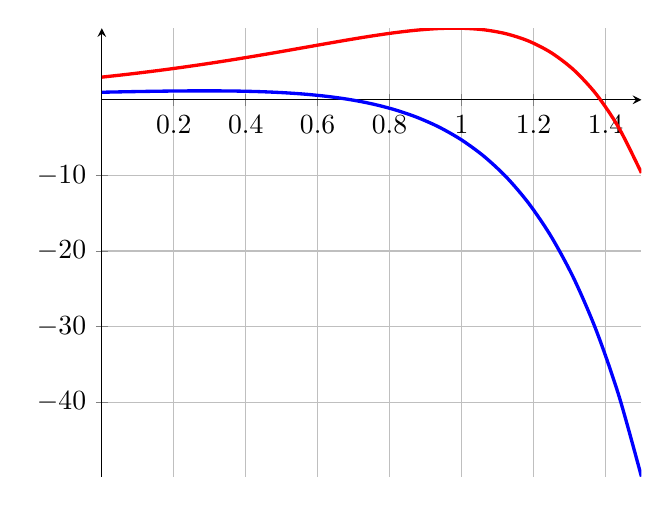
\begin{tikzpicture}
        \begin{axis}[axis lines=center, domain=0:1.5, xmin=0, xmax=1.5, grid]
            \addplot[smooth, very thick, blue] {2*exp(2*x) - exp(3*x)};
            \addplot[smooth, very thick, red] {4*exp(2*x) - exp(3*x)};
        \end{axis}
    \end{tikzpicture}
\end{center}
}

% \begin{problem}
%     \begin{itemize}
%             \input{ClickerQuestions/DEQ.10.20.030}
%     \end{itemize}
% \end{problem}


\begin{problem}
    Since we know that both $x_1=x_2=e^{3t}$ and $x_1=e^{-t}, x_2=-e^{-t}$ are solutions
    to the system 
    \begin{flalign*} 
        x_1' & =  x_1  +2x_2 \\ x_2' & = & 2x_1  + x_2 \\
    \end{flalign*} 
    Which of the following are also solutions?
\begin{enumerate}
    \item[(a)] 
\begin{flalign*}
    x_1 & =  3e^{3t}-e^{-t} \\
    x_2 & =  3e^{3t}+e^{-t} \\
  \end{flalign*} 
\item[(b)] 
\begin{flalign*}
    x_1 & =  -e^{3t}-e^{-t} \\
    x_2 & =  -e^{3t}+e^{-t} \\
  \end{flalign*} 

\item[(c)] 
\begin{flalign*}
     x_1 & =  2e^{3t}+4e^{-t} \\
    x_2 & = -4e^{-t}+2e^{3t} \\
  \end{flalign*} 

\item[(d)] 
\begin{flalign*}
    x_1 & =  0 \\
    x_2 & =  0 \\
\end{flalign*} 

\item[(e)] None of the above

\item[(f)] All of the above.

\end{enumerate}


\end{problem}
% \begin{problem}
%     \begin{itemize}
%             \input{ClickerQuestions/DEQ.10.20.040}
%     \end{itemize}
% \end{problem}



\begin{problem}
    Consider the system of differential equations,

\[
y'(t) = \left( 
\begin{array}{ccc}
14 & 0 & -4 \\
2 & 13 & -8 \\
-3 & 0 & 25 \\
\end{array}
\right) y(t)
\].

Which of the following functions solve this system?
\begin{enumerate}
    \item[(a)]
        $y(t) = \left( \begin{array}{c} 1 \\ 0 \\ 3 \\ \end{array} \right) e^{-4 t}$
    \item[(b)]
        $y(t) = \left( \begin{array}{c} 1 \\ 3 \\ 2 \\ \end{array} \right) e^{6 t}$
    \item[(c)]
        $y(t) = \left( \begin{array}{c} 4 \\ 0 \\ 1 \\ \end{array} \right) e^{13 t}$
    \item[(d)] None of the above
    \item[(e)] All of the above.
\end{enumerate}

\end{problem}
% \begin{problem}
%     \begin{itemize}
%             \input{ClickerQuestions/DEQ.10.20.050}
%     \end{itemize}
% \end{problem}

% \begin{problem}
%     \begin{itemize}
%             \input{ClickerQuestions/DEQ.10.22.100}
%     \end{itemize}
% \end{problem}

\begin{problem}\label{prob:linear_fighting}
    Two forces are fighting one another. Let $x$ and $y$ be the number of soldiers in each
    force and let $a$ and $b$ be the offensive fighting capacities of $x$ and $y$ respectively.
    Assume that forces are lost only to combat, and no reinforcements are brought in.
    \begin{enumerate}
        \item[(a)] Write a system of differential equations that models this scenario.
            Write the system as a matrix equation.
        \item[(b)] Solve the system using the eigenvalue method using sensible initial
            conditions and values for $a$ and $b$.
        \item[(c)] Determine values of $a$ and $b$ for which army $x$ wins and for which
            army $y$ wins.
    \end{enumerate}
\end{problem}


\begin{problem}\label{prob:linear_fighting_nonhom}
    In Problem \ref{prob:linear_fighting} we built a model that might be really good for
    hand-to-hand combat.  Let's tweak this model.
    \begin{enumerate}
        \item[(a)] Modify the model from Problem \ref{prob:linear_fighting} to allow each
            army to get a constant number of recruits each day (assume time is measured in
            days).
        \item[(b)] Propose a solution technique for this model and implement it.
        \item[(c)] Propose a way to find a steady state solution to your model (if it
            exists) and implement your idea.
    \end{enumerate}
\end{problem}

% \begin{problem}
%     \begin{itemize}
%             \input{ClickerQuestions/DEQ.10.19.010}
%     \end{itemize}
% \end{problem}

In a linear system where there is a constant non-homogeneity we need to modify our solution
technique.  Consider the system of differential equations
\begin{flalign}
    \bx'(t) = A \bx + \bb
    \label{eqn:nonhomog_linear_system}
\end{flalign}
where $\bx$ is a vector of functions, $A$ is a real matrix, and $\bb$ is a vector of
constants.  Problem \ref{prob:linear_fighting_nonhom} should result in a model of this
type and in that problem you proposed a solution technique and a method for finding the
steady-state solution.  Now let's summarize these techniques.
\begin{technique}
    Let $\bx$ be an $n\times n$ vector of single variable functions, let $A$ be an $n\times n$ real matrix, and let
    $\bb$ be an $n \times n$ real vector.  Consider the system of $n$ differential
    equations
    \[ \bx' = A \bx + \bb \]
    with initial conditions $\bx(0) = \bx_0$. Observe that this is a non-homogeneous
    differential equation with a constant non-homogeneity.  The general solution
    to the differential equation is
    \[ \bx(t) = \underline{\hspace{2in}} \]
    where \ldots (complete the technique)
\end{technique}
\solution{
    \[ \bx(t) = \sum_{j=1}^n c_j \left( \bv_j e^{\lambda_j t} \right) + \bw \]
    where $\bw$ is the steady state vector resulting from solving the equation $A \bw +
    \bb = \bo$ and the constants arise from the equation $\bx_0 - \bw = \sum_{j=1}^n c_j \bv_j$
}

\begin{problem}
    Consider the linear system of differential equations given by
    \[ \begin{pmatrix} x' \\ y' \end{pmatrix} = \begin{pmatrix} -3 & 1 \\ 0 & -3
        \end{pmatrix} \begin{pmatrix} x \\ y \end{pmatrix} + \begin{pmatrix} 3 \\ 6
    \end{pmatrix} \]
    with initial conditions $x(0) = 1$ and $y(0) = 0$.  Solve the system of equations,
    generate a plot of the solution, and find the steady state (if it exists).
\end{problem}

\begin{problem}
    Solve the second order differential equation $y'' + 4y' + 3y = 2$ by converting to a
    first order system.  Find the equilibrium if it exists.
\end{problem}
\solution{
Partial solution:\\
Let $x = y'$ and we can rewrite as
\begin{flalign*}
    x' &= -4y + 3x + 2 \\
    y' &= x
\end{flalign*}
which can be rewritten as 
    \[ \begin{pmatrix} x' \\ y' \end{pmatrix} = \begin{pmatrix} 3 & -4 \\ 1 & 0
        \end{pmatrix} \begin{pmatrix} x \\ y \end{pmatrix} + \begin{pmatrix} 2 \\ 0
    \end{pmatrix} \]
    The equilibrium can be found by solving
    \[ \begin{pmatrix} 0 \\ 0 \end{pmatrix} = \begin{pmatrix} 3 & -4 \\ 1 & 0
        \end{pmatrix} \begin{pmatrix} x \\ y \end{pmatrix} + \begin{pmatrix} 2 \\ 0
    \end{pmatrix} \]
}




\section{The Matrix Exponential}
Recall that if we are solving the first order linear homogeoneous differential equation
$x' = rx$ we know (from separation of variables) that the solution is $x(t) = x_0 e^{rt}$.
This is one of the simplest ordinary differential equation that there is!  In this chapter we
have encountered linear systems of differential equations that have a very similar form:
\begin{flalign}
    \bx' = A \bx
    \label{eqn:linear_system_matrix_eqn}
\end{flalign}
where $\bx$ this time is a vector of functions and $A$ is a matrix of values.  More
clearly, if $A$ is an $n \times n$ real matrix then a linear system of differential
equations can be written as
\[ \begin{pmatrix} x_1'(t) \\ x_2'(t) \\ \vdots \\ x_n'(t) \end{pmatrix} = \begin{pmatrix}
        a_{11} & a_{12} & \cdots & a_{1n} \\
        a_{21} & a_{22} & \cdots & a_{2n} \\
    \vdots & \vdots & \ddots & \vdots \\
a_{n1} & a_{n2} & \cdots & a_{nn} \end{pmatrix} \begin{pmatrix} x_1(t) \\ x_2(t) \\ \vdots
\\ x_n(t) \end{pmatrix}. \]
It stands
to reason that the solution to \eqref{eqn:linear_system_matrix_eqn} should be the same, or
at least have the same form, as the solution to the simple differential equation $x' =
rx$.  Hence we conjecture that the solution to \eqref{eqn:linear_system_matrix_eqn} is
\begin{flalign}
    \bx = e^{A t} \bx_0
    \label{eqn:linear_system_matrix_eqn_soln}
\end{flalign}
where $\bx_0$ is the vector of initial conditions. \ldots but wait!  What is $e^{At}$?
That's right, we have a matrix in the exponent of an exponential function!

To understand the matrix exponential we first start by recalling the Taylor series of the
exponential function
\[ e^x = 1 + x + \frac{x^2}{2} + \frac{x^3}{3!} + \frac{x^4}{4!} + \cdots. \]
If instead we examine the function $f(x) = e^{ax}$ where $a \in \mathbb{R}$ then it is
easy to see that
\[ e^{ax} = 1 + ax + a^2 \frac{x^2}{2} + a^3 \frac{x^3}{3!} + a^4 \frac{x^4}{4!} + \cdots.
\]

If we use the Taylor series as the definition of the exponential function then a natural
definition for the matrix exponential is as follows.
\begin{definition}[Matrix Exponential]
    Let $A$ be a square matrix and $t$ be a real variable.  The matrix exponential
    $e^{At}$ is defined as
    \begin{flalign}
        e^{At} = I + At + A^2 \frac{t^2}{2} + A^3 \frac{t^3}{3!} + A^4 \frac{t^4}{4!} +
        \cdots.
        \label{eqn:matrix_exponential_Taylor}
    \end{flalign}
\end{definition}
Recall that if $A$ has a complete collection of eigenvalues and eigenvectors
then we can find matrices $P$ and $D$ such that $A = PDP^{-1}$.  Therefore the definition
of the matrix exponential can be rewritten as
\begin{flalign}
    \notag e^{At} &= I + PDP^{-1}t + PD^2P^{-1} \frac{t^2}{2} + PD^3P^{-1} \frac{t^3}{3!} +
    PD^4P^{-1} \frac{t^4}{4!} + \cdots \\
    &= P \left(  I + Dt + D^2 \frac{t^2}{2} + D^3 \frac{t^3}{3!} + D^4 \frac{t^4}{4!} +
    \cdots \right) P^{-1} 
    \label{eqn:matrix_exponential_Taylor_Eigen}
\end{flalign}


Using either \eqref{eqn:matrix_exponential_Taylor} or
\eqref{eqn:matrix_exponential_Taylor_Eigen} we now have a way to find the analytic
solution to a linear homogeneous system of differential equations of the form $\bx' = A
\bx$.  

\begin{thm}\label{thm:system_soln_matrix_exp}
    If $\bx$ is a vector of functions and $A$ is a real square matrix then the solution to
    the differential equation $\bx' = A \bx$ is
    \[ \bx(t) = e^{At} \bx_0. \]
\end{thm}

The computation of the matrix exponential in Theorem \ref{thm:system_soln_matrix_exp} is
potentially really obnoxious by hand, but thankfully there are built-in tools for
performing the computation in the most scientific computing software.  For example, in
MATLAB you can use the command \mcode{expm(A)} to find the matrix exponential of the matrix
$A$.

\begin{example}
    Use the matrix exponential to solve the system of differential equations 
    \[ \bx'(t) = \begin{pmatrix} 2 & 0 \\ 1 & 2 \end{pmatrix} \bx(t) \quad \text{with}
        \quad \begin{pmatrix} x_1(0) \\ x_2(0) \end{pmatrix} = \begin{pmatrix} 2 \\ -3
    \end{pmatrix} \]
    {\bf Solution:} The following MATLAB code finds the matrix exponential
\begin{lstlisting}
clear; clc;
syms t
A = [2 , 0 ; 1 , 2];
x0 = [2;-3];
x = expm(A*t) * x0   % this is the solution to the system of ODEs
\end{lstlisting}
    which results in the solution 
    \[ \begin{pmatrix} x_1(t) \\ x_2(t) \end{pmatrix} = \begin{pmatrix} e^{2t} & 0 \\
        te^{2t} & e^{2t} \end{pmatrix} \begin{pmatrix} 2 \\ -3 \end{pmatrix}. \]
    pulling this out of matrix form we have
    \[ x_1(t) = 2e^{2t} \quad \text{and} \quad x_2(t) = 2te^{2t} - 3e^{2t}. \]
    Finally we can plot the solution with the following code.
\begin{lstlisting}
tmax = 1;
ezplot(x(1),[0,tmax])
hold on
ezplot(x(2),[0,tmax])
axis([0,1,-10,10])
\end{lstlisting}
\end{example}
Hint: You can use
the command \mcode{latex(simplify(x))} to take your symbolic answer for $\bx(t)$ from MATLAB and get it into \LaTeX.

The following two problems give you a chance to practice using the matrix exponential to
solve applied systems of differential equations problems.  Have fun!!

\begin{problem}
    Tank \#1 is connected to Tank \#2 by two separate pipes.  Pure water is flowing
    into Tank \#1 at a rate of 2 gallons per minute.  Tank \#1 is initially filled with 50
    gallons of water with 5 pounds of salt dissolved in it.  Tank \#2 contains 40 gallons
    of water with 1 pound of salt dissolved in it.  Solution flows from Tank \#1 to Tank
    \#2 at a rate of 3 gallons per minute and from Tank \#2 to Tank \#1 and at a rate of 1
    gallon per minute.  Thoroughly mixed solution is also being drained from Tank \#2 at a
    rate of 2 gallons per minute.  Let $x(t)$ be the amount of salt in Tank \#1 and let
    $y(t)$ be the amount of salt in Tank \#2 at time $t$.  
    \begin{enumerate}
        \item[(a)] Write the linear system of differential equations that models this
            scenario. Be sure to include your initial conditions (it may help to draw a
            picture first).
        \item[(b)] Solve the system of differential equations using the matrix
            exponential.  Clearly write your answer in matrix and  vector form.
        \item[(c)] Solve the system again using the eigenvalue method.  Clearly write your
            answer showing how the eigenvalues and eigenvectors play a role in the
            solution.
        \item[(d)] Make a plot showing how the two concentrations evolve over 100 minutes.
    \end{enumerate}
\end{problem}




\begin{problem}
    You are given a mechanical system with three springs $A$, $B$, and $C$ and two
    objects $F$ and $G$ each of mass $M$.  Springs $A$ and $C$ have spring constant
    $k$ and spring $B$ has spring constant $2k$.  Spring $A$ is attached to a wall on
    the left and spring $C$ is attached to a wall on the right. Let $x_1(t)$ be the
    position of $F$ from it's equilibrium ($x_1=0$ indicates that $F$ is at
    equilibrium), and let $x_2(t)$ be the position of $G$ from it's equilibrium.  See
    Figure \ref{fig:double_spring_mass}.
    \begin{figure}[ht!]
        \begin{center}
            \begin{tikzpicture}
                \tikzstyle{ground}=[fill,pattern=north east lines,draw=none,minimum width=0.3,minimum height=0.6]
                \tikzstyle{sky}=[fill,pattern=north east lines,draw=none,minimum width=0.3,minimum height=0.6]

                \node (wall1) [ground, minimum height=2cm] {};
                \draw (wall1.north east) -- (wall1.south east);
                \node [draw,minimum width=0.5cm,minimum height=0.5cm] (massF) at (3,0) {$F$};
                \node [draw,minimum width=0.5cm,minimum height=0.5cm] (massG) at (5,0) {$G$};
                \node (rightend) at (8,0) [sky,minimum height=2cm] {};
                \draw (rightend.south west) -- (rightend.north west);
                \node (fix) at (0,0) {};
                \draw [
                    snake=coil,
                    segment amplitude=5pt,
                    segment length=5pt
                ] (wall1.east) -- (massF); 
                \draw [
                    snake=coil,
                    segment amplitude=5pt,
                    segment length=5pt
                ] (massF.east) -- (massG.west); 
                \draw [
                    snake=coil,
                    segment amplitude=5pt,
                    segment length=5pt
                ] (massG.east) -- (rightend.west); 
                \draw [
                    thick,
                    decoration={
                        brace,
                        mirror,
                        raise=0.5cm
                    },
                    decorate
                ] (wall1.east) -- (massF) 
                node [pos=0.5,anchor=north,yshift=-0.55cm] {$A$}; 
                \draw [
                    thick,
                    decoration={
                        brace,
                        mirror,
                        raise=0.5cm
                    },
                    decorate
                ] (massF.east) -- (massG.west) 
                node [pos=0.5,anchor=north,yshift=-0.55cm] {$B$}; 
                \draw [
                    thick,
                    decoration={
                        brace,
                        mirror,
                        raise=0.5cm
                    },
                    decorate
                ] (massG.east) -- (rightend) 
                node [pos=0.5,anchor=north,yshift=-0.55cm] {$C$}; 
            \end{tikzpicture}
        \end{center}
        \caption{Double spring mass system}
        \label{fig:double_spring_mass}
    \end{figure}
    
    Initial conditions: Assume that we move mass $F$ exactly 1 unit to the
            left and let it go.  This means that $x_1(0) = -1$ and $x_3(0) = x_1'(0) = 0$.
            If we initially hold mass $G$ fixed then $x_2(0)=x_4(0)=0$.    
    \begin{enumerate}
        \item[(a)] First we'll write the second order linear system of equations.  This system of
            equations is just a statement of Hooke's law for springs: $F = -kx$, where $k$ is
            the spring constant.  To help you get
            started you can use the skeleton below:
            \begin{flalign*}
                M x_1'' &= -k x_1 + \left( \text{some spring constant} \right) \left(
                \text{distance between $x_2$ and $x_1$}
                \right) \\
                M x_2'' &= -2k \left( x_2 - x_1 \right) - \left( \text{some spring constant}
                \right) x_2
            \end{flalign*}


        \item[(b)] To turn this into a first-order system we introduce two new variables: $x_3 =
            x_1'$ and $x_4 = x_2'$.  Write this system of differential equations \dots I'll
            get you started \dots
            \begin{flalign*}
                x_1' &= x_3 \\
                x_2' &= x_4 \\
                x_3' &= \text{ \dots } \\
                x_4' &=  \text{ \dots }
            \end{flalign*}
            Now write the system as a matrix equation of the form $\frac{d\bx}{dt} = A \bx$.

        \item[(c)] Solve the linear system of differential equations with the method of
            matrix exponentials.
        \item[(d)] Next solve the linear system of differential equations with the
            eigenvalue method. You {\it should} find that you have 4 purely imaginary
            eigenvalues (I'll wait while you let MATLAB find these for you \dots).  This
            means that you will have oscillations in your solutions. Why?
%         
% 
%         
%         Hence, if we let $\lambda_j = \alpha_j
%         i$ then $e^{\lambda_j t} = \cos(\alpha_j t) + i\sin(\alpha_j t)$ by Euler's
%         formula.  Therefore, the solution to the system of differential equations becomes
%         \begin{flalign*} \bx(t) &= \left( A_1 \cos(\alpha_1 t) + B_1 \sin(\alpha_1 t)
%             \right) \bv_1 \\
%             &\quad+\left( A_2 \cos(\alpha_2 t) + B_2 \sin(\alpha_2 t) \right) \bv_2 \\
%             &\quad+\left( A_3 \cos(\alpha_3 t) + B_3 \sin(\alpha_3 t) \right) \bv_3 \\
%             &\quad+\left( A_4 \cos(\alpha_4 t) + B_4 \sin(\alpha_4 t) \right) \bv_4.
%         \end{flalign*}
%         You should have values of $\alpha_1, \alpha_2, \alpha_3,$ and $\alpha_4$ as well
%         as the eigenvectors $\bv_1, \bv_2, \bv_3$, and $\bv_4$.

        \item[(e)] Plot your solutions.
    \end{enumerate}
\end{problem}


\section{Complex Eigenvalues}
In this brief section we consider the case where the eigenvalues of the coefficient matrix
in a linear system are complex.  If $\bx' = A \bx$ and $A$ has complex eigenvalues
$\lambda = \alpha \pm \beta i$ then the solution to the system is
\[ \bx(t) = C_1 e^{\lambda_1 t} \bv_1 + C_2 e^{\lambda_2 t} \bv_2 = e^{\alpha t} \left(
C_1 e^{\beta i t} \bv_1 + C_2 e^{-\beta i t} \bv_2 \right). \]
If we use Euler's formula for the complex exponentials the solution becomes
\[ \bx(t) = e^{\alpha t} \left( C_1 \left( \cos(\beta t) + i\sin(\beta t) \right) \bv_1 +
C_2 \left( \cos(\beta t) - i\sin(\beta t) \right) \bv_2 \right). \]
Now if we gather the trigonometric functions the solution can be written as
\begin{flalign} \bx(t) = e^{\alpha t} \left[ \left( C_1 \bv_1 + C_2 \bv_2 \right) \cos(\beta t) +
\left( C_1 i \bv_1 - C_2 i \bv_2 \right) \sin(\beta t)
\right].\label{eqn:linear_system_oscillations}
\end{flalign}
Form the initial conditions we know that $\bx(0) = C_1 \bv_1 + C_2 \bv_2$ and once we have
calculated $C_1$ and $C_2$ it is straight forward to find the vectors multiplying the
cosine and sine terms in the solution.

\begin{example}\label{ex:linear_system_oscillation}
    Solve the system of differential equations 
    \[ \bx'(t) = \begin{pmatrix} -2 & -2 \\ 2 & -2 \end{pmatrix} \bx(t) \]
    with initial condition $\bx(0) = \begin{pmatrix} 3 \\ -3 \end{pmatrix}$. \\
    {\bf Solution:} We first need to find the eigenvalues and eigenvectors of the
    coefficient matrix, $A$.  
    \[ \bv_1 = \begin{pmatrix} -i \\ -1 \end{pmatrix} \quad \text{with} \quad \lambda_1 =
    -2 + 2i \]
    \[ \bv_2 = \begin{pmatrix} i \\ -1 \end{pmatrix} \quad \text{with} \quad \lambda_2 =
    -2 - 2i \]
    Solve the system of equation $\begin{pmatrix} \bv_1 \, \bv_2 \end{pmatrix}
    \begin{pmatrix} C_1 \\ C_2 \end{pmatrix} = \bx(0)$ to get $C_1 = \frac{3}{2} +
    \frac{3}{2} i$ and $C_2 = \frac{3}{2} - \frac{3}{2} i$ (the actual computation is left
    to the reader). 
    Hence,
    \[ C_1 \bv_1 + C_2 \bv_2 = \left( \frac{3}{2} + \frac{3}{2} i \right) \begin{pmatrix}
        -i \\ -1 \end{pmatrix} + \left( \frac{3}{2} - \frac{3}{2}i \right) \begin{pmatrix}
    i \\ -1 \end{pmatrix} = \cdots = \begin{pmatrix} 3 \\ -3 \end{pmatrix}  \]
    and
    \[ C_1i \bv_1 - C_2i \bv_2 = \left( \frac{3}{2} + \frac{3}{2} i \right)i \begin{pmatrix}
        -i \\ -1 \end{pmatrix} - \left( \frac{3}{2} - \frac{3}{2}i \right)i \begin{pmatrix}
    i \\ -1 \end{pmatrix} = \cdots = \begin{pmatrix} 3 \\ 3 \end{pmatrix}  \]
    Now we can substitute into \eqref{eqn:linear_system_oscillations} to get the complete
    solution
    \[ \bx(t) = e^{-2t} \left( \cos(2t) \begin{pmatrix} 3 \\ -3 \end{pmatrix} + \sin(2t)
    \begin{pmatrix} -3 \\ 3 \end{pmatrix} \right) = \begin{pmatrix} e^{-2t} \left( 3
        \cos(2t) + 3 \sin(2t)
    \right) \\ e^{-2t} \left( -3\cos(2t) + 3\sin(2t) \right) \end{pmatrix}. \]
    The solutions to the system are shown in Figure \ref{fig:linear_system_oscillation}
\end{example}

\begin{figure}
    \begin{center}
        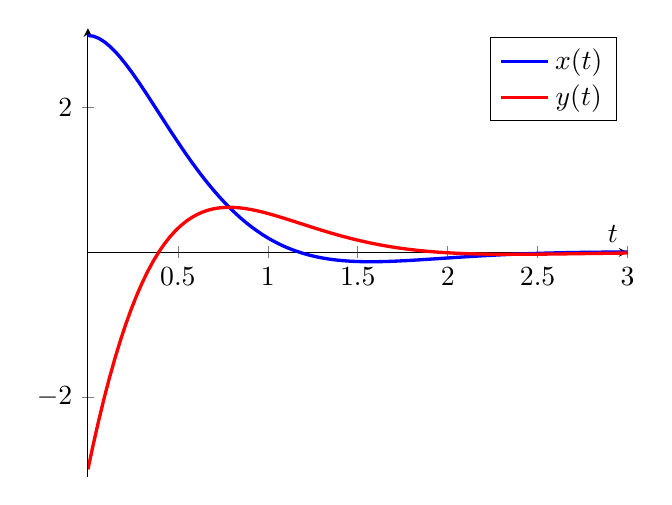
\begin{tikzpicture}
            \begin{axis}[axis lines=center, domain=0:3, xmin=0, xmax=3, ymin=-3.1, ymax=3.1,
                xlabel={$t$}]
                \addplot[blue, very thick, samples=100] {exp(-2*x)*(3*cos(2*deg(x)) + 3*sin(2*deg(x)))};
                \addlegendentry{$x(t)$};
                \addplot[red, very thick, samples=100] {exp(-2*x)*(-3*cos(2*deg(x)) + 3*sin(2*deg(x)))};
                \addlegendentry{$y(t)$};
            \end{axis}
        \end{tikzpicture}
    \end{center}
    \caption{Solution curves for Example \ref{ex:linear_system_oscillation}}
    \label{fig:linear_system_oscillation}
\end{figure}


\section{Additional Exercises}
